\documentclass[a4paper]{article}

\usepackage[utf8]{inputenc}
\usepackage[portuguese]{babel}
\usepackage{graphicx}
\usepackage{a4wide}
\usepackage[pdftex,hidelinks]{hyperref}
\usepackage{float}
\usepackage{indentfirst}
\usepackage{subcaption}
\usepackage[cache=false]{minted}
\usepackage{amsmath}
\usepackage{listings}
\usepackage{color}

\definecolor{dkgreen}{rgb}{0,0.6,0}
\definecolor{gray}{rgb}{0.5,0.5,0.5}
\definecolor{mauve}{rgb}{0.58,0,0.82}

\lstset{frame=tb,
  language=C++,
  aboveskip=3mm,
  belowskip=3mm,
  showstringspaces=false,
  columns=flexible,
  basicstyle={\small\ttfamily},
  numbers=none,
  numberstyle=\tiny\color{gray},
  keywordstyle=\color{blue},
  commentstyle=\color{dkgreen},
  stringstyle=\color{mauve},
  breaklines=true,
  breakatwhitespace=true,
  tabsize=3
}
\begin{document}

\title{Computação Gráfica\\ Primitivas gráficas}
\author{Bárbara Cardoso (a80453) \and Marcio Sousa (a82400) \and Pedro Mendes (a79003)}
\date{\today}

\begin{titlepage}

    %título
    \thispagestyle{empty}
    \begin{center}
        \begin{minipage}{0.75\linewidth}
            \centering
            %engenharia logo
            
\includegraphics[width=0.4\textwidth]{eng.jpeg}\par\vspace{1cm}
            \vspace{1.5cm}
            %títulos
            \href{https://www.uminho.pt/PT}{\scshape\LARGE Universidade do Minho} \par
            \vspace{1cm}
            \href{https://www.di.uminho.pt/}{\scshape\Large Departamento de Informática} \par
            \vspace{1.5cm}

            \maketitle
        \end{minipage}
    \end{center}

\end{titlepage}

\tableofcontents

\pagebreak

\section{Introdução}
Este trabalho foi proposto no âmbito da unidade curricular de Computação Gráfica, e tem como objetivo desenvolver um motor gráfico genérico para representar objetos a 3 dimensões.

O projeto está dividido em várias fases, sendo que nesta primeira, serão implementadas algumas primitivas gráficas, como o plano, o paralelepípedo, a esfera e o cone e também uma primeira implementação de dois modos de Câmera.

\section{Arquitetura do Projecto}
Após analisar o problema, foi decidido que o projeto está dividido em dois executáveis, o \texttt{generator} e o \texttt{engine}. Para além destes, temos também na nossa arquitetura uma biblioteca comum aos dois.

\subsection{Common}

Aqui está apenas defindo um \texttt{Point.cpp/hpp} que representa um ponto no espaço 3D.

\subsection{Engine}

Este modulo é composto pelo \texttt{model.cpp/hpp} que representa cada modelo, ou seja, cada conjunto de pontos, disponibilizando também um método para o desenhar. E a \texttt{main.cpp} que carrega todos os ficheiros especificados no ficheiro \texttt{config.xml} e desenha-os no ecrã. Esta define também a lógica que controla a camera.

\subsection{Generator}

Este modulo é composto pelo \texttt{generator.cpp/hpp} que disponibiliza metodos para gerar os pontos necessários para desenhar as 4 primitivas geométricas e a \texttt{main.cpp} que interpreta os argumentos da linha de comandos para chamar estes métodos e produzir um ficheiro com estes.

\section{Primitivas}
 Para esta fase do projeto foram desenhadas quatro figuras, contando com um plano, um cubo, uma esfera e um cone. Serão a seguir apresentados os algoritmos apresentados para o cálculo dos pontos necessários para desenhar cada uma dessas primitivas, bem como uma contextualização com as premissas utilizadas durante o raciocínio, quando necessário.
\subsection{Plano}
\begin{figure}[H]
\centering
\includegraphics[width=0.5\linewidth]{plano.png}
\caption{Plano: args = ....}
\end{figure}

O plano é um figura de extrema simplicidade, constando de 6 pontos que constituem 2 triângulos, que por sua vez criarão o plano em XoZ.



É recebido como parâmetro o comprimento do lado do quadrado em questão, que será usado para calcular os pontos. Sendo que este plano estará centrado na origem, cada um dos pontos é calculado da seguinte forma:
\\
\begin{figure}[H]
\centering
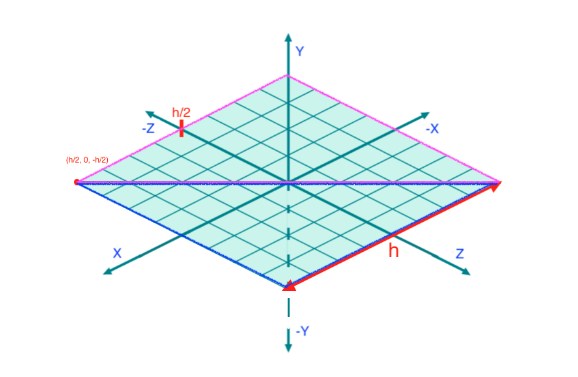
\includegraphics[width=0.5\linewidth]{esquemaPlano.PNG}
\caption{Esquema do Plano.}
\end{figure}
\pagebreak

Para o triângulo superior:\\
\\
-  \texttt{h/2, 0, h/2}\\
-  \texttt{-h/2, 0, -h/2}\\
-  \texttt{-h/2, 0, h/2}\\
\\
Para o triângulo inferior:\\
\\
-  \texttt{-h/2, 0, -h/2}\\
-  \texttt{h/2, 0, h/2}\\
-  \texttt{h/2, 0, -h/2}\\
\\
Com base nisto, temos então o algoritmo usado para o cálculo dos pontos.\\
\begin{lstlisting}
std::vector<Point*> draw_plane(double side_length){
    vector<Point*> coordsPlane;
    float axis = side_length / 2;

    //first triangle
    coordsPlane.push_back(new Point(axis, 0, axis));
    coordsPlane.push_back(new Point(-axis, 0, -axis));
    coordsPlane.push_back(new Point(-axis, 0, axis));

    //second triangle
    coordsPlane.push_back(new Point(-axis, 0, -axis));
    coordsPlane.push_back(new Point(axis, 0, axis));
    coordsPlane.push_back(new Point(axis, 0, -axis));

    return coordsPlane;
}

\end{lstlisting}

\subsection{Paralelepípedo}
\begin{figure}[H]
\centering
\includegraphics[width=0.5\linewidth]{paralelicoiso.png}
\caption{Paralelepípedo: args = ....}
\end{figure}

Um paralelepípedo é formado por 6 faces, sendo cada face formada por $divisions^2$ quadrados, sendo cada um desses quadrados formado por dois triângulos. Estas divisões são utilizadas para iterar sobre todas as superfícies do paralelepípedo, sendo esta distância entre divisões usada para calcular o próximo ponto baseado no ponto "atual". \\
\\

Tendo o paralelepípedo centrado na origem por motivos de facilidade de cálculos, calculamos:\\
\\
\texttt{double axisX = x / 2;}\\
\texttt{double axisY = y / 2;}\\
\texttt{double axisZ = z / 2;}\\

como "valores máximos" que podem ser tomados por cada uma das coordenadas dos pontos que constituem o paralelepípedo, e\\
\\
\texttt{double spacingX = x / divisions;}\\
\texttt{double spacingY = y / divisions;}\\
\texttt{double spacingZ = z / divisions;}\\

como sendo os valores que, tal como o nome indica, correspondem ao espaçamento entre divisões para cada eixo.\\

Para calcular todos os pontos foi feito uso do seguinte algoritmo:\\
\\
\begin{lstlisting}
std::vector<Point*> draw_box(double x, double y, double z, int divisions){
    vector<Point*> coordsBox;
    double axisX = x / 2;
    double axisY = y / 2;
    double axisZ = z / 2;
    double spacingX = x / divisions;
    double spacingY = y / divisions;
    double spacingZ = z / divisions;

    for (int i = 0; i < divisions; i++) {
        for (int k = 0; k < divisions; k++) {
            //Front
            coordsBox.push_back(new Point(-axisX + spacingX * i, -axisY + spacingY * k, axisZ));
            coordsBox.push_back(new Point(-axisX + spacingX * (i + 1), -axisY + spacingY * k, axisZ));
            coordsBox.push_back(new Point(-axisX + spacingX * i, -axisY + spacingY * (k + 1), axisZ));
            coordsBox.push_back(new Point(-axisX + spacingX * (i + 1), -axisY + spacingY * k, axisZ));
            coordsBox.push_back(new Point(-axisX + spacingX * (i + 1), -axisY + spacingY * (k + 1), axisZ));
            coordsBox.push_back(new Point(-axisX + spacingX * i, -axisY + spacingY * (k + 1), axisZ));

            //Back
            coordsBox.push_back(new Point(-axisX + spacingX * i, -axisY + spacingY * k, -axisZ));
            coordsBox.push_back(new Point(-axisX + spacingX * i, -axisY + spacingY * (k + 1), -axisZ));
            coordsBox.push_back(new Point(-axisX + spacingX * (i + 1), -axisY + spacingY * k, -axisZ));
            coordsBox.push_back(new Point(-axisX + spacingX * (i + 1), -axisY + spacingY * k, -axisZ));
            coordsBox.push_back(new Point(-axisX + spacingX * i, -axisY + spacingY * (k + 1), -axisZ));
            coordsBox.push_back(new Point(-axisX + spacingX * (i + 1), -axisY + spacingY * (k + 1), -axisZ));

            //Up
            coordsBox.push_back(new Point(-axisX + spacingX * i, axisY, -axisZ + spacingZ * k));
            coordsBox.push_back(new Point(-axisX + spacingX * i, axisY, -axisZ + spacingZ * (k + 1)));
            coordsBox.push_back(new Point(-axisX + spacingX * (i + 1), axisY, -axisZ + spacingZ * (k + 1)));
            coordsBox.push_back(new Point(-axisX + spacingX * i, axisY, -axisZ + spacingZ * k));
            coordsBox.push_back(new Point(-axisX + spacingX * (i + 1), axisY, -axisZ + spacingZ * (k + 1)));
            coordsBox.push_back(new Point(-axisX + spacingX * (i + 1), axisY, -axisZ + spacingZ * k));

            //Down
            coordsBox.push_back(new Point(-axisX + spacingX * i, -axisY, -axisZ + spacingZ * k));
            coordsBox.push_back(new Point(-axisX + spacingX * (i + 1), -axisY, -axisZ + spacingZ * (k + 1)));
            coordsBox.push_back(new Point(-axisX + spacingX * i, -axisY, -axisZ + spacingZ * (k + 1)));
            coordsBox.push_back(new Point(-axisX + spacingX * i, -axisY, -axisZ + spacingZ * k));
            coordsBox.push_back(new Point(-axisX + spacingX * (i + 1), -axisY, -axisZ + spacingZ * k));
            coordsBox.push_back(new Point(-axisX + spacingX * (i + 1), -axisY, -axisZ + spacingZ * (k + 1)));

            //Left
            coordsBox.push_back(new Point(-axisX, -axisY + spacingY * i, -axisZ + spacingZ * k));
            coordsBox.push_back(new Point(-axisX, -axisY + spacingY * i, -axisZ + spacingZ * (k + 1)));
            coordsBox.push_back(new Point(-axisX, -axisY + spacingY * (i + 1), -axisZ + spacingZ * k));
            coordsBox.push_back(new Point(-axisX, -axisY + spacingY * (i + 1), -axisZ + spacingZ * k));
            coordsBox.push_back(new Point(-axisX, -axisY + spacingY * i, -axisZ + spacingZ * (k + 1)));
            coordsBox.push_back(new Point(-axisX, -axisY + spacingY * (i + 1), -axisZ + spacingZ * (k + 1)));

            //Right
            coordsBox.push_back(new Point(axisX, -axisY + spacingY * i, -axisZ + spacingZ * k));
            coordsBox.push_back(new Point(axisX, -axisY + spacingY * (i + 1), -axisZ + spacingZ * k));
            coordsBox.push_back(new Point(axisX, -axisY + spacingY * i, -axisZ + spacingZ * (k + 1)));
            coordsBox.push_back(new Point(axisX, -axisY + spacingY * (i + 1), -axisZ + spacingZ * k));
            coordsBox.push_back(new Point(axisX, -axisY + spacingY * (i + 1), -axisZ + spacingZ * (k + 1)));
            coordsBox.push_back(new Point(axisX, -axisY + spacingY * i, -axisZ + spacingZ * (k + 1)));
        }
    }

    return coordsBox;
}
\end{lstlisting}
\subsection{Esfera}

\begin{figure}[H]
\centering
\includegraphics[width=0.5\linewidth]{bolinha.png}
\caption{Esfera: args=....}
\end{figure}

Uma esfera é dividida em stacks e slices, que serão usadas para iterar a toda a volta da mesma. A interseção entre as slices e as stacks forma retângulos, e cada um desses retângulos será formado por dois triângulos.


Para a criação da esfera serão usadas coordenadas esféricas devido à facilidade que proporcionam no caso em questão. Assim sendo, são necessárias duas variáveis para representar os dois ângulos que constituem este tipo de coordenadas, \texttt{Phi} e \texttt{Theta}, utilizadas na iteração.

\begin{figure}[H]
\centering
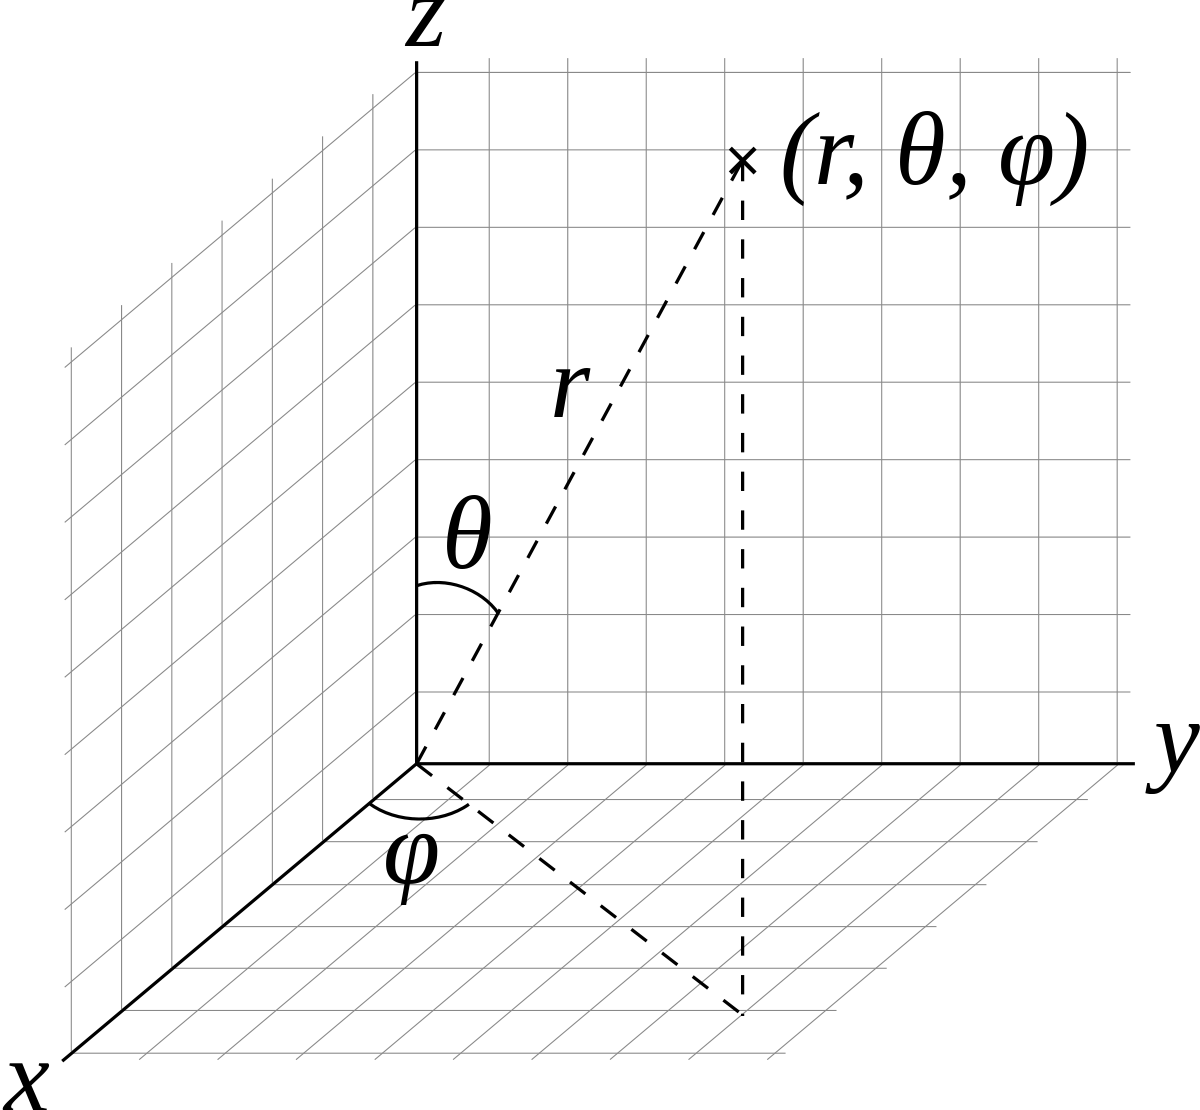
\includegraphics[width=0.5\linewidth]{coords.png}
\caption{Coordenadas esféricas.}
\end{figure}

Para cálculo das coordenadas de cada ponto será também necessário calcular a stack e slice em que se encontram atualmente as iterações, \texttt{currentStack} e \texttt{currentSlice} que serão calculadas da seguinte forma:\\
\\
\texttt{float currentStack = theta * thetaMovement}\\
\texttt{float currentSlice = phi * phiMovement}\\
\\

As variáveis \texttt{thetaMovement} e \texttt{phiMovement} correspondem respetivamente à distância entre Stacks e à distância entre Slices.\\
\\
\texttt{float phiMovement = M\_PI * 2 / slices;}\\
\texttt{float thetaMovement = M\_PI / stacks;}\\
\\

Para utilizar coordenadas esféricas, o X, Y e Z devem ser alterados, passando a ser:\\
\\
\texttt{x = radius * sin(theta) * sin(phi);}\\
\texttt{y = radius * cos(theta);}\\
\texttt{z = radius * sin(theta) * cos(phi);}\\

O algoritmo de cálculo dos pontos para desenhar uma esfera é a seguir apresentado.\\
\\
\begin{lstlisting}
std::vector<Point*> draw_sphere(double radius, double slices, double stacks){
    vector<Point*> coordsSphere;

    float phiMovement = M_PI * 2 / slices;

    float thetaMovement = M_PI / stacks;

    for (float phi = 0; phi < slices; phi++)
        for (float theta = 0; theta < stacks; theta++) {

            float currentStack = theta * thetaMovement;
            float currentSlice = phi * phiMovement;

            coordsSphere.push_back(new Point(radius * sin(currentStack + thetaMovement) * sin(currentSlice + phiMovement),
                radius * cos(currentStack + thetaMovement),
                radius * sin(currentStack + thetaMovement) * cos(currentSlice + phiMovement)));

            coordsSphere.push_back(new Point(radius * sin(currentStack) * sin(currentSlice),
                radius * cos(currentStack),
                radius * sin(currentStack) * cos(currentSlice)));

            coordsSphere.push_back(new Point(radius * sin(currentStack + thetaMovement) * sin(currentSlice),
                radius * cos(currentStack + thetaMovement),
                radius * sin(currentStack + thetaMovement) * cos(currentSlice)));

            coordsSphere.push_back(new Point(radius * sin(currentStack) * sin(currentSlice + phiMovement),
                radius * cos(currentStack),
                radius * sin(currentStack) * cos(currentSlice + phiMovement)));

            coordsSphere.push_back(new Point(radius * sin(currentStack) * sin(currentSlice),
                radius * cos(currentStack),
                radius * sin(currentStack) * cos(currentSlice)));

            coordsSphere.push_back(new Point(radius * sin(currentStack + thetaMovement) * sin(currentSlice + phiMovement),
                radius * cos(currentStack + thetaMovement),
                radius * sin(currentStack + thetaMovement) * cos(currentSlice + phiMovement)));
        }

    return coordsSphere;
}

\end{lstlisting}

\subsection{Cone}

\begin{figure}[H]
\centering
\includegraphics[width=0.5\linewidth]{insertConeHerePlease.png}
\caption{Cone: args = ....}
\end{figure}

O cone tem a base sobre o eixo XoZ, centrada na origem, e é dividido em stacks e slices. A função geradora dos pontos do cone recebe como parâmetros o raio, a altura, o número de slices e o número de stacks.

São declaradas três variáveis, \texttt{phi}, \texttt{theta} e \texttt{stackSpacing}.
\\

A primeira corresponde à divisão equivalente da base por cada slice.
\\
\\


\texttt{float phi = (2 * M\_PI) / slices;}\\
\\

A segunda, \texttt{theta}, é calculada dividindo o raio da base pelo numero de stacks, o que se traduz na prática a calcular o recuo do raio à medida que se sobe nas stacks.
\\
\\

\texttt{float theta = radius / stacks;}\\
\\

Por fim, \texttt{stackSpacing}, tal como o nome indica, corresponde à distância entre cada stack, o "stack shift", e é calculado dividindo a altura pelo número de stacks.\\
\\


\texttt{float stackSpacing = height / stacks;}\\
\\

O desenho do cone em si foi dividido em 3 fases: Base, Topo e a zona em volta, e tal como na esfera, são utilizadas coordenadas esféricas.

Para a base, quando estamos na primeira stack, em cada iteração é desenhado um triângulo, e conjunto destes triângulos desenhados formarão a base concêntrica na origem quando tiverem sido executadas todas as iterações.

O topo é desenhado no fim, para completar a "ponta" do cone, então, quando estamos na penúltima stack(a última é o vértice do cone), são desenhados triângulos a toda a volta que partilham um ponto em comum (o vértice), um por cada slice.

Para os lados, com exceção do topo, serão desenhados retângulos formados por dois triângulos cada um, e serão esses retângulos que constituem o cone até chegar ao topo.
\\
Esta lógica traduzida para código resultou no seguinte algoritmo:
\\
\begin{lstlisting}
std::vector<Point*> draw_cone(double radius, double height, int slices, int stacks){
    vector<Point*> coordsCone;
    float phi = (2 * M_PI) / slices;
    float stackSpacing = height / stacks;
    float theta = radius / stacks;

    for (int i = 0; i < stacks; i++) {
        for (int k = 0; k < slices; k++) {

            if (!i) {
                //Base
                coordsCone.push_back(new Point(0, 0, 0));
                coordsCone.push_back(new Point(radius * sin(phi * (k + 1)), 0, radius * cos(phi * (k + 1))));
                coordsCone.push_back(new Point(radius * sin(phi * k), 0, radius * cos(phi * k)));
            }

            if (i == stacks - 1) {
                //Top
                coordsCone.push_back(new Point((radius - theta * i) * sin(phi * k), i * stackSpacing, (radius - theta * i) * cos(phi * k)));
                coordsCone.push_back(new Point((radius - theta * i) * sin(phi * (k + 1)), i * stackSpacing, (radius - theta * i) * cos(phi * (k + 1))));
                coordsCone.push_back(new Point(0, stacks * stackSpacing, 0));
            }

            else { //Around
                coordsCone.push_back(new Point((radius - theta * i) * sin(phi * k), i * stackSpacing, (radius - theta * i) * cos(phi * k)));
                coordsCone.push_back(new Point((radius - theta * (i + 1)) * sin(phi * (k + 1)), (i + 1) * stackSpacing, (radius - theta * (i + 1)) * cos(phi * (k + 1))));
                coordsCone.push_back(new Point((radius - theta * (i + 1)) * sin(phi * k), (i + 1) * stackSpacing, (radius - theta * (i + 1)) * cos(phi * k)));
                coordsCone.push_back(new Point((radius - theta * i) * sin(phi * k), i * stackSpacing, (radius - theta * i) * cos(phi * k)));
                coordsCone.push_back(new Point((radius - theta * i) * sin(phi * (k + 1)), i * stackSpacing, (radius - theta * i) * cos(phi * (k + 1))));
                coordsCone.push_back(new Point((radius - theta * (i + 1)) * sin(phi * (k + 1)), (i + 1) * stackSpacing, (radius - theta * (i + 1)) * cos(phi * (k + 1))));
            }
        }
    }

    return coordsCone;
}

\end{lstlisting}

\section{Câmera}
A Câmera pode ser utilizada em dois modos diferentes, o modo \textit{Explorer mode} e o modo \textit{FPS mode}, que podem ser alternados durante a execução do engine.

\subsection{Explorer Mode}

Neste modo o movimento da Câmera é descrito por uma superfície esférica, na qual o utilizador se movimenta enquanto mantém, sempre, o seu olhar fixo na origem do referencial. O raio desta superfície esférica é que define a distância até ao centro, podendo ser aumentado para afastar o utilizador do centro do espaço 3d, ou diminuído para o aproximar.

\subsubsection{Controlos \textit{(key bindings)}}

\begin{itemize}
    \item \texttt{H}: Move no plano xz no sentido ao dos ponteiros do relógio.
    \item \texttt{J}: Desce.
    \item \texttt{K}: Sobe.
    \item \texttt{L}: Move no plano xz no sentido contrário ao dos ponteiros do relógio.
    \item \texttt{I}: Reduz o raio da esfera.
    \item \texttt{O}: Aumenta o raio da esfera.
\end{itemize}

\subsection{FPS Mode}

Neste modo a posição da câmera no espaço 3d é completamente livre, assim o utilizador pode mover-se em linha reta em qualquer direção. Pode também alterar o ponto para o qual está a olhar na horizontal e na vertical.

\subsubsection{Controlos \textit{(key bindings)}}

\begin{itemize}
    \item \texttt{W}: Move para a frente.
    \item \texttt{A}: Move para a esquerda.
    \item \texttt{S}: Move para trás.
    \item \texttt{D}: Move para a direita.
    \item \texttt{H}: Olha para a esquerda.
    \item \texttt{J}: Olha para baixo.
    \item \texttt{K}: Olha para cima.
    \item \texttt{L}: Olha para a direita.
    \item \texttt{G}: Desce.
    \item \texttt{Shift+G}: Sobe.
\end{itemize}

\subsection{Transição de modos de câmera}

Para que a transição seja \textit{smooth} foi necessário converter de um sistema de coordenadas para o outro.

Quando a câmera se encontra no modo \textit{Explorer} a sua posição é determinada pelo vetor definido através dos ângulos $\alpha$ e $\beta$ e através da distância à origem. E o ponto para onde está a olhar é a origem. Logo para efectuar a transição para \textit{FPS} foi necessário encontrar um vector que quando aplicado na posição da camera, olhe para a origem.

\begin{figure}[H]
    \[
        \alpha_f =
        \begin{cases}
            \alpha_e + \pi & \quad \text{se } \alpha_e < 0\\
            \alpha_e - \pi & \quad \text{caso contrario}
        \end{cases}
    \]
    \[
        \beta_f = -\beta_e
    \]
    \caption{Transição de \textit{Explorer} para \textit{FPS}.}
\end{figure}

Quando a câmera se encontra no modo \textit{FPS} é necessário encontrar o ângulos $\alpha$ e $\beta$ e o raio. Estes definem o vetor correspondente às coordenadas (\texttt{(x,y,z)}) da câmera no momento da transição.

\begin{figure}[H]
    \[
        \alpha_e =
        \begin{cases}
            \arctan(x / z)       & \quad \text{se } z < 0\\
            \arctan(x / z) + \pi & \quad \text{caso contrario}
        \end{cases}
    \]
    \[
        \beta_e = \arcsin\bigg(\frac{y}{\sqrt{x^2 + y^2 + z^2}}\bigg)\\
    \]
    \[
        radius = \sqrt{x^2 + y^2 + z^2}
    \]
    \caption{Transição de \textit{FPS} para \textit{Explorer}.}
\end{figure}

\subsection{Outros controlos \textit{(key bindings)}}

\begin{itemize}
    \item \texttt{+}: Aumenta a escala de todos os modelos.
    \item \texttt{-}: Diminui a escala de todos os modelos.
    \item \texttt{V}: Muda o modo da câmera.
    \item \texttt{Q}: Termina o programa.
\end{itemize}

\section{Conclusões e Trabalho Futuro}
Em suma, todas as primitivas são geradas corretamente e o motor gráfico é capaz de as representar genericamente.

Futuramente, a câmera será melhorada para que se possa utilizar o rato no modo \textit{FPS}.

\end{document}



